\documentclass[bachelor,14pt,subf,href,colorlinks=true
%,times        % шрифт Times как основной
%,fixint=false % отключить прямые знаки интегралов
]{disser}

\usepackage[
  a4paper, mag=1000, includefoot,
  left=3cm, right=1cm, top=2cm, bottom=2cm, headsep=1cm, footskip=1cm
]{geometry}
\usepackage[T2A]{fontenc}
\usepackage[utf8]{inputenc}
\usepackage{graphicx}
\usepackage[english,russian]{babel}
\ifpdf\usepackage{epstopdf}\fi

% Номера страниц сверху и по центру
%\def\headfont{\small}
%\pagestyle{headcenter}
%\chapterpagestyle{empty}

% Точка с запятой в качестве разделителя между номерами цитирований
%\setcitestyle{semicolon}

% Использовать полужирное начертание для векторов
\let\vec=\mathbf

% Включать подсекции в оглавление
\setcounter{tocdepth}{2}

\graphicspath{{figure/}}

\begin{document}

\institution{Московский физико-технический институт (государственный университет)\\Физтех-школа физики и исследований им. Ландау\\ОП Вычислительная физика конденсированного состояния и живых систем\\Объединенный институт высоких температур РАН}

% Имя лица, допускающего к защите (зав. кафедрой)
\apname{Норман Г.Э.}

\title{Выпускная квалификационная работа\\[-14pt]на соискание степени\\БАКАЛАВРА}

\topic{Молекулярно-Динамическая модель \\ кристалла Лизоцима}

% Автор
\author       {Поляченко Юрий Анатольевич} % ФИО
\group        {786} % Группа
\coursenum    {03.03.01} % Номер направления
\course       {Прикладные математика и физика}

% Научный руководитель
\sa      {Стегайлов В.В.}
\sastatus{д.~ф.-м.~н., в.~н.~с.}
% Второй научный руководитель
%\sasnd      {ФИО руководителя}
%\sasndstatus{д.~ф.-м.~н., ст.~н.~с.}

% Рецензент
%\rev      {Храпак А.Г.}
%\revstatus{д.~ф.-м.~н., г.~н.~с.}
% Второй рецензент
%\revsnd      {ФИО рецензента}
%\revsndstatus{д.~т.~н., ст.~н.~с.}

% Консультант
%\con{ФИО консультанта}
%\conspec{вопросам\\охраны труда}
%\constatus{к.~т.~н., доц.}
% Второй консультант
%\consnd{ФИО консультанта}
%\consndspec{экономическим\\вопросам}
%\consndstatus{к.~э.~н., доц.}

% Город и год
\city{Москва}
\date{\number\year}

\maketitle

%%
%% Titlepage in English
%%
%
%\institution{Name of Organization}
%
%% Approved by
%\apname{Professor S.\,S.~Sidorov}
%
%\title{Master's Thesis}
%
%% Topic
%\topic{Dummy Title}
%
%% Author
%\author{Author's Name} % Full Name
%\course{Physics} % Название специальности
%
%\group{} % Study Group
%\masterprog   {Title of program}
%
%% Scientific Advisor
%\sa       {I.\,I.~Ivanov}
%\sastatus {Professor}
%
%% Reviewer
%\rev      {P.\,P.~Petrov}
%\revstatus{Associate Professor}
%
%% Consultant
%\con{}
%\conspec{}
%\constatus{}
%
%% City & Year
%\city{Saint Petersburg}
%\date{\number\year}
%
%\maketitle[en]

\tableofcontents

\intro

\textbf{������������ ������.} � ��������� ����� ��� ���� ���������� ����� ���������� ��������������� ����������������� ��������� ��������� ��������. ����� ����� ����� ���������� ������� ������, ������ ��������� ��������� �������� � ��� ���� �� ��������� ���������� ����������. ������ ������-����� �������� ���������� �������� � �������� �����������������. �������� �������� � ��� ����� ��������� ���������� ������� ������������ � ������������� � ������������ �� ������ �������. ������ �������� � �� �� ����� ���������� ������� ������������ ������, ������� ���� ���� ���� ������������ �������������� �������� ������� ������ ��������� ���� ������ ����� ������.

\textbf{���� ������} �������� � ���, ����� ����������� ������� ������������ ������ ������-����� � � �������� ����� �� ��������� � ��������� � �������� ���������.

������ ������� �� ��� ���� � ����������.

� ����� \ref{Sec:MTF} ���������� �������������� ������ ������-�����, ���������� �������� ������������� �������� � ��������� ��� ���������� �������.

� ����� \ref{Sec:Calculation} �������������� � ������� ������� �������� ��������� ������.

� ����� \ref{Sec:Results} ��������� ���������� ��������� �������� � ���������� �������.

� ���������� ������ ����������� ���������� ���������� � �������� ��������������� ������.

\chapter{������ ������-����� ��� ������� � �������� ������������ � �������� � ���}
\label{Sec:MTF}

� ���� ����� ���������� �������� � �������� ������ ������-����� (���) � � ����������� �������� --- ������ ������-����� � ���������� (����).

� ������� \ref{Subsec:electron} ���������� �������� �������� �� ��������� ���� ����������, � ����� �� �� �������� � �������������� ��������������.

� ������� \ref{Subsec:MTF} �������������� ��� ����� �������������� �������� ������ � ��������� �������� ��������� ��� ���������� �������.

� ������� \ref{Subsec:MTF-corrections} �������������� � ����������� �������� ������ � ���������, ������� ��������� ������ �������������� �������. ���������� ����� �. �. �������� ��������� ��������� ��������, � ����� ����������� ������������ ������� ������������ ������.

� ������� \ref{Subsec:thermodynamics} ����������� ����� ��������� ��� �������� ����������������� �������, ������������ ��� ��������� ��������.

� ������� \ref{Subsec:thermal_contribution} �������������� � �������, ��������� � ���������� �� ����������������� ������� �������� �����.

\section{��������� ��� ��������� ����������}
\label{Subsec:electron}

��������� ����������� ���������� �����-������
\begin{equation}
  n = \frac{1}
      {
        \mathrm{exp}\,
        (
          \frac
            {\varepsilon - \mu}
            {T}
        )
        +
        1
      }
  \label{eq:fermi_dirac}
\end{equation}
� ����� 2 �������� �������� ���������. ��� ������� ����������� �������������
��������� ��� ���������
\begin{equation}
  n(\varepsilon)
  =
  \Theta(\mu - \varepsilon)
  =
  \begin{cases}
    1, & \varepsilon < \mu, \\
    0, & \varepsilon > \mu. \\
  \end{cases}
\end{equation}
��� $ T = 0 $ ������������ $ \mu(T = 0) = \varepsilon_F $ ���������� �������� �����. ��������� ������������ ������� ��������� $ \varepsilon = p^2/2m $, ��� ����� ���������, ������ �� ������� �� ������ ����� ������ � ������� ������� $ V $:
$$
  N
  =
  2V
  \int
  \Theta(\varepsilon_F - \varepsilon)
  \frac{d^3p}
  {(2\pi\hbar)^3}
  =
  \frac{V}{\pi^2\hbar^3}\int_0^{\varepsilon_F}\frac12(2m)^{3/2}\sqrt{\varepsilon}d\varepsilon
  =
  \frac{V}{3\pi^2\hbar^3}(2m\varepsilon_F)^{3/2}.
$$
����� �������,
\begin{equation}
  \varepsilon_F = \frac{\hbar^2}{2m}\left(3\pi^2 n\right)^{2/3},
\end{equation}
� ������� ������������ ������� ���������:
$$
  <\varepsilon>
  =
  2V
  \int \varepsilon
  \Theta(\varepsilon_F - \varepsilon)
  \frac{d^3p}
  {(2\pi\hbar)^3}
  =
  \frac35 \varepsilon_F
  \sim
  n^{2/3}.
$$

� ����� ������ ������������ ������������ �� �������
$$
  N
  =
  2V
  \int
  \frac{1}
      {
        \mathrm{exp}\,
        (
          \frac
            {\varepsilon - \mu}
            {T}
        )
        +
        1
      }
  \frac{d^3p}
  {(2\pi\hbar)^3}.
$$

%��������� ������ �� $ n $ ������������ ����������, �������� ��� ������ ������������ �������
%�������
%\begin{equation}
%  E_K
%  = \int n(\mathbf r) <\varepsilon> d^3r
%  = \frac35 \frac{\hbar^2}{2m}(3\pi^2)^{2/3}\int n^{5/3}(\mathbf r)d^3r
%  \label{eq:E_K_zero}
%\end{equation}

�� ����� �� ������������ ��������� ��������������������. �� ����� ����, ����� ����������� ���� ������������������ ��������������, �������, � ����������� �� �������� ��������� ����������, �������� � ���� ������ ��������� ��������.

��-������, ��������� � ����� �������� ��������� � ���� �������� ������� �����, �� ����� ��������� � ����� ���������������� ���������, � ������ ����� ������ ����������� ��������� ���������������� ����������, ������� �������� � ���������� �� ������������������� ��������������. ��� �������������� ������� �������� ��������, � ��� �������� ��� ��� ������������� ���������� ������������������� ������������.

��-������, ��������� � ������ �������� ���������� ����� ������������� ���������� ������ ���� � �����, �� ������������������ ������������ ����� ���� �������� ������ ������ �� �� ���������������� ����������. ���� ������ ������� �������� �����������.

� ����� \cite{Gambosh:1951} �������, ��� ����� ������ ��� ������� � ���� �������� 1-�� ������� ������ ����������, � �������� ��� ����� �������� �������� ������� � ����������. ����� ������������� ������������� ��� ���������� � ���� ������� ����
$$
  \psi_j(\mathbf r) = \frac{1}{\sqrt{V}}e^{i(\mathbf k_j, \mathbf r)}.
$$
� ����������� �� ����������� ������, �������� ������� ������� ���� ���������� ����� ���� ���� ������������, ���� ���������������� �� ������������:
$$
  \begin{aligned}
  \psi_s = \frac{1}{\sqrt{2}}\left[\psi_i(1)\psi_j(2) + \psi_j(1)\psi_i(2)\right], \\
  \psi_a = \frac{1}{\sqrt{2}}\left[\psi_i(1)\psi_j(2) - \psi_j(1)\psi_i(2)\right].
  \end{aligned}
$$
����������, ��� ������� �� N ���������� ����� ��������� �� ��� �����, � ������ �� ������� ��� ����������� �����. ��� ������ ������ ���������� �������� ������� $ \psi^{(1)} $, $ \psi^{(2)} $ ����� �������� � ���� ������������ ��������, � ���������� --- � ���� ������������ �������� ������� ������ �� ����� $ \psi = \psi^{(1)}\psi^{(2)} $. ������������� ��������� ������� ��������� � ����� ���� ��� ���������� �������� �� ����������� ������� � ������ ������� ������ ����������:
$$
  \delta E = <\psi|\frac12\sum_{i,j = 1}^N\frac{e^2}{|\mathbf r_i - \mathbf r_j|}|\psi >.
$$
������������� ������������� ��������� ������ ����� ��������� ���������� ��������� � ����������� ����������
$$
  \rho_{ij}(\mathbf r)
  =
  \psi_i(\mathbf r)\psi_j^*(\mathbf r)
  =
  \frac{1}{V}e^{i(\mathbf k_i - \mathbf k_j) \mathbf r},
$$
��� ���� �������� �������� ������� ���� ���������� �� ����� ������
$$
  A_{ij} = e^2\iint\frac{\rho_{ij}(\mathbf r)\rho^*_{ij}(\mathbf r')}{|\mathbf r - \mathbf r'|}d^3rd^3r'.
$$
����� ������������� ���������
$$
  V_{ij}(\mathbf r) = \int\frac{\rho^*_{ij}(\mathbf r')}{|\mathbf r - \mathbf r'|}d^3r'
$$
��� ��������� ������������� ����������� ��������� $ \rho^*_{ij} $. ����� ����� ��������� ��������
$$
  \Delta V_{ij} = -4\pi e \rho^*_{ij}(\mathbf r) = -\frac{4\pi}{V}e^{-i(\mathbf k_i - \mathbf k_j) \mathbf r},
$$
������ �������, ���
$$
  V_{ij}(\mathbf r)
  =
  \frac{4\pi e}{|\mathbf k_i - \mathbf k_j|^2}\rho^*_{ij}(\mathbf r)
  =
  \frac{4\pi\hbar^2 e}{|\mathbf p_i - \mathbf p_j|^2}\rho^*_{ij}(\mathbf r),
$$
� �������� �������
\begin{equation}
  A_{ij}
  = e^2\int\rho_{ij}(\mathbf r)V_{ij}(\mathbf r)d^3r
  = \frac{4\pi\hbar^2 e^2}{|\mathbf p_i - \mathbf p_j|^2} \frac{1}{V}.
  \label{eq:exchange_energy}
\end{equation}

%����� �������� Gambosh, ��� ������ �������� ������� $ N $ ����������
%\begin{equation}
%  A = -\frac{4\pi e^2 V}{h^4}p^4_F
%\end{equation}

������ ������� ���������� ���� ��������� ���������� ��� ������ �������� \cite{Wigner:PR:1934}. �� ������� ��������� ����������� ���������:
\begin{equation}
  W_c = - \frac{\alpha_1}{n^{1/3} + \alpha_2}n^{1/3}
  \label{eq:correlation_energy}
\end{equation}
���
$$
  \alpha_1 = 0,05647\frac{e^2}{a_0}, \quad \alpha_2 = 0,1216\frac{1}{a_0}.
$$
\section{������ ������-�����}
\label{Subsec:MTF}

� �������������� ������ ������ \cite{Thomas:PCPS:1926} � ����� \cite{Fermi:RAL:1927} �������������� ����������� ����������� ��� � ����������������� �����������. ����� ������� ��������� ������������� ���������� �������������, � ����������� ������ ������������������ �������������� ���������� � ������ � ���� � ������. ������� ������������ ����, ����� �������, �������� ������������ ����������� ���������. �������� ��������� ����������, ����� �������� �� ����������� ������������, ���������� �������� �������.

� ������ \cite{Feynman:PR:1949} ���� �������� ������ ���������� ��� �������� ����������. �������� ��������� ��� ������������������ ���������� ����� ������ �� ������������� ��������. � ����� \cite{Nikiforov:2000} �� �������� ��������� �������� ������� ����������� ������������� ���������� � ����������������� ����:
\begin{equation}
  f(\mathbf r, \mathbf p)
  =
  \frac{1}{\mathrm{exp}
            \left(
              \frac{p^2/2m_e - V(\mathbf r) - \mu}{T}
            \right) + 1},
\end{equation}
�, ��������������, ����������� ������������ ����������
$$
  n_e(\mathbf r)
  =
  \frac{2}{(2\pi\hbar)^3}
  \int_0^\infty
  \frac{4\pi p^2dp}
       {\mathrm{exp}
            \left(
              \frac{p^2/2m_e - V(\mathbf r) - \mu}{T}
            \right) + 1}
  =
$$
\begin{equation}
  =
  \frac{(2m_eT)^{3/2}}{2\pi^2}
  I_{1/2}
  \left(
    \frac{V(\mathbf r) + \mu}{T}
  \right),
\end{equation}
��� �����, ���������� ����� ������� �����-������, � ��� ������� ����������� ��������� �
$$
  n_0(\mathbf r)
  =
  \frac{2}{(2\pi\hbar)^3}
  \int_0^{\mu + V(\mathbf r)}2\pi(2m_e)^{3/2}\sqrt{\varepsilon}d\varepsilon
  =
  \frac{1}{3\pi^2}\left[\frac{2m_e}{\hbar^2}(V(\mathbf r) + \mu)\right]^{3/2},
$$
��� � � �������������� ������� ������ � �����.

��� ������� � \cite{Kirzhnits:SPU:1975}, ������� ��������� �������� ��� ������������������ ���������� ����������� ����������, ���� ��������������� ������� ����������� ����� �������-������. �������� ����������� �� ������������ ����������� �����, ������ �� ������� �������� ���� ���� � � ����� �����������������. ��������� ������� ���������� ������ ������ $ r_0 $:
$$
  \int_{r < r_0} n(\mathbf r) d^3r = Z.
$$
����� �������, ����� ������� � ���������� ������������ ������������� ������ � ������ ������-����� � ���������� ���������:
\begin{equation}
  \left\{
  \begin{aligned}
    \Delta V = 4\pi e &n_e(\mathbf r) = \frac{2e}{\pi}(2m_eT)^{3/2}
    I_{1/2}
    \left(
      \frac{V(\mathbf r) + \mu}{T}
    \right), \\
    \left.rV(r)\right|_{r = 0} &= eZ, \quad V(r_0) = 0, \\
    \left.\frac{dV}{dr}\right|_{r = r_0} =& 0.  \\
  \end{aligned}
  \right.
\end{equation}
�������� � ������� �������� � ����� ������ $ r_0x = r$, $ \phi(x)/x = (V(r) + \mu)/T)$, �������� ������� ������:
\begin{equation}
  \left\{
  \begin{aligned}
    \frac{d^2\phi}{dx^2} &= \frac{4}{\pi}\sqrt{2T}r_0^2xI_{1/2}\left(\frac{\phi}{x}\right), \\
    \phi(0) &= \frac{Z}{r_0T}, \quad \phi '(1) = \phi(1).
  \end{aligned}
  \right.
  \label{eq:MTF_nonzero}
\end{equation}

\section{�������� � ������ ������-����� � ������� � ������������}
\label{Subsec:MTF-corrections}

��� ��� ���� ��������, ������������� ���� ������ ��������� ������ ������������������ �������������� ����� ����������� � �����. ����� ����, ������� ������ ���� ���������� ����������. ����� �������������� ������� ����� ������� �� ��������� �������� ��� ������������������ ����������:
$$
  \frac{p_{\mu}^2}{2m_e} + V(\mathbf r) = const,
$$
\begin{equation}
  -\Delta V = \Delta \frac{p_{\mu}^2}{2m_e} = 4\pi n \simeq \frac{1}{L^2}\frac{p_{\mu}^2}{2m_e}
  \Rightarrow
  L \sim \frac{p_{\mu}}{\sqrt{n}}.
  \label{eq:irregularity}
\end{equation}
���, ��� ����������� ������� ������� $ L $, �������� ����������� ��������� �������.

��� ���������� � \ref{Subsec:electron}, ��������� � ������������� ������� ��������� ������ ���� �� �����. ������ �� ���������� $ \sim \lambda \sim 1/p_{\mu} $, ������� ����������� ���������� �������������� ����� ����
$$
  \left(
    \frac{\lambda}{L}
  \right)^2V
  \sim
  \frac{n}{p^2_{\mu}},
$$
� ��������, ������ ��������� ������� ������ � ������������
\begin{equation}
  \delta_{\mathrm{exc}} \sim \frac{n}{p^4_{\mu}},
\end{equation}
���������� ������������� ����� �������� ��������. ������ �������� �������������� ������� ���� ������ ������� \cite{Dirac:PCPS:1930}. �������� �������� ������� ���������� ���� ���������� \eqref{eq:exchange_energy} � �������� � � ������ �������, �� ������� �������� � ����������� ������������ ���������� � ��������� ������-�����-������.

��� ���� �������� ���������� ����� ����������: ��������� ������� ������������ �������������� � ������������ �������:
$$ \delta \sim \frac{n^{1/3}}{p_{\mu}^2}. $$
���������� ��������� �� ������ ������� ������ ����������, ������� ����� �������� ���� �������� � �������, �� ������ ����������� ������������ �� ������� �����������, ������� ���������� �� �������� ������� ������� �����:
$$
  Ln^{1/3} \sim \delta^{-1/2}
$$
� ��������� ������� ��������� ���������� $ \delta $.
����� �������, �������� ���������� ������� �� ������� ���������� ������������ ����. ������� ���������� ������������ ���������� ������� ����� � ����������� $ \sim n^{2/3}/T $. � ������� ���������� ������������ �� �������� ��������� �� �������� ��������� $ \delta $, ������� � ������� ����������
$$
  n^{2/3} \gg T, \quad p_{\mu} \sim n^{1/3}, \quad \delta \sim n^{-1/3},
$$
� �������� ����� ���:
$$
  \delta_{\mathrm{exc}} \sim n^{-1/3}, \quad \delta_{\mathrm{cor}} \sim n^{-2/3}.
$$
��� ������������� ������������ ����:
$$
  n^{2/3} \ll T, \quad p_{\mu} \sim T^{1/2}, \delta \sim n^{1/3}/T,
$$
� ������������ ����� �����, ��� $ \delta_{\mathrm{cor}} = \delta^{3/2} $.
�������
$$
  \delta_{\mathrm{exc}} \sim n/T^2, \quad \delta_{\mathrm{cor}} \sim n^{1/2}/T^{3/2}.
$$
����� ���������� ���������� ������ \cite{Gombas:ZP:1943}.

���, ��� �������� �������� ������� �������, �������� ������� ������� ������������ �� ��������� � ���� ���������.
\begin{figure}[h!]
  \label{region_of_applic}
  \center{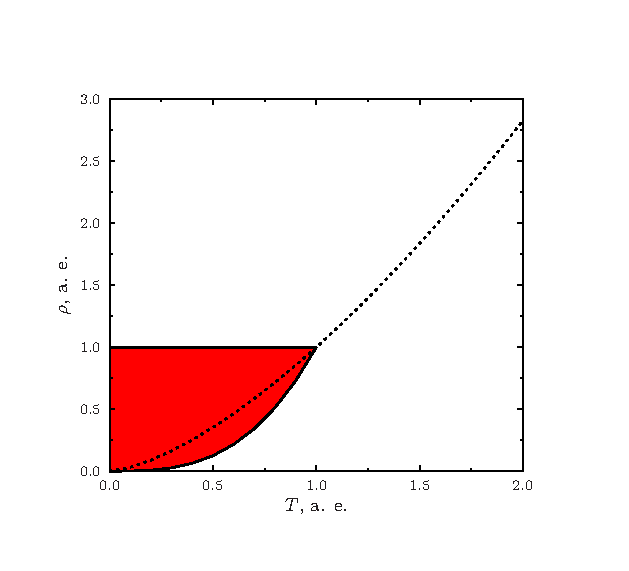
\includegraphics[scale=1.4]{region_of_applicability.eps}}
  \caption{
  ������� ������������ ������ ������-�����. � �������, ���������� �������, ����������� ��������� �������, � ��� ������ �����������. ��������� ���������� ������ ����������: ���� ������ ��� ��������, ���� --- ����������.}
\end{figure}

��� ����� �� ����������� �������� ������ ������-����� ���� ������������� � ������ �������������� ����������, ��� ���������� � ���������������� �������� �� ����. ��� ���� ������ ������������ \cite{Weizsacker:ZP:1935} � ���� ��� ���������� ����������� ��������. ������� ��������� � �������� ��������� (������ ����) ����������� ��� �������� �������� ������� �, ��� �����, ���������� ����� �������� ����������� ���������.

�� ��� ��������������� ������� � ��������� ����� ���� ������ �. �. ��������� \cite{Kirzhnits:JETP:1957}. �� ���������������� ���������� ������ � ����������� ����. �������� ������� ���������, ������������ ���, ���
$$
  \hat \rho \psi_n = \rho_n \psi_n,
$$
��� $ \rho_n $ --- ������� ���������� ������ $ n $, � ������ ���������� �����-������ ����� ���:
\begin{equation}
  \hat \rho (\hat H) = \frac{1}{1 + \mathrm{exp}\left(\frac{\hat H - \mu}{T}\right)},
\end{equation}
� ���� ���������
\begin{equation}
  \rho(\mathbf r) = \int e^{-i\mathbf p \mathbf r/\hbar}\hat \rho(\hat H)
  e^{-i\mathbf p \mathbf r/\hbar} \frac{2d^3p}{(2\pi\hbar)^3}.
\end{equation}

������������ ����������� ������� � ������ ��������� �������������� ����� ���
$$
  \hat H = \frac{\hat p^2}{2m_e} - eV(\mathbf r) - \hat A,
$$
��� �������� ��������� �������������� $ A $ � ������� \eqref{eq:exchange_energy} ����� ����������� ���:
\begin{equation}
  \hat A(\mathbf r, \hat{\mathbf p})
  =
  \int
  e^{-i\mathbf p \mathbf r/\hbar}
  \frac{4\pi\hbar^2e^2\hat \rho(\hat H')}{|\mathbf p - \mathbf p'|^2}
  e^{i\mathbf p' \mathbf r/\hbar}
  \frac{d^3p}{(2\pi\hbar)^3}.
\end{equation}

�������� ��������� $ \hat \rho $ �� ������� $ e^{i\mathbf p \mathbf r/\hbar} $ ����� ������ � �������� �� $ 1 $ ������� �������� �� $ \mathbf p - i\hbar\nabla $. ����� �������, ��� ����� ������
$$
  \hat \rho(\hat H) = \frac{(\mathbf p - i\hbar\nabla)^2}{2m_eT} - \frac{V(\mathbf r) + \mu}{T} = \hat \rho(\hat a + \hat b).
$$
�������� $ \rho $ �� ������������:
\begin{multline}
  \rho(\hat a + \hat b) = \rho(a + b) + \frac12[\hat a, \hat b]\rho''(a + b) + \\
  +\frac16\left([\hat a,[\hat a, \hat b]] + [[\hat a, \hat b],\hat b]\right)\rho'''(a + b) + \frac18([\hat a, \hat b])^2\rho^{IV}(a + b) + ...
\end{multline}
��������� $ \Phi = (V + \mu)/T $ � �������� ��� �����������, ������� ��� ���������� ���������:
$$
  e^{-i\mathbf p \mathbf r/\hbar}\hat \rho(\hat H)e^{-i\mathbf p \mathbf r/\hbar}
  =
  \rho(\varepsilon) + \frac{i\hbar}{2m_eT}\rho''(\varepsilon)\mathbf p \nabla\Phi
   + \frac{\hbar^2}{4m_eT}\rho''(\varepsilon)\Delta \Phi -
$$
\begin{equation}
   - \frac{\hbar^2}{6m_eT}\rho'''(\varepsilon)(\nabla \Phi )^2 + \frac{\hbar^2}{6(m_eT)^2}\rho'''(\varepsilon)(\mathbf p \nabla)^2\Phi - \frac{\hbar^2}{8(m_eT)^2}\rho^{IV}(\varepsilon)(\mathbf p \nabla\Phi)^2,
\end{equation}
��� $ \varepsilon = p^2/(2m_eT) - (V(\mathbf r) + \mu)/T $. ����� �������������� ��������� ������ ����� ���������� ������� $ \hbar^2 $.

�������� � ��������� �� ���� ������ ����� ��������� ��� (� ������� ��������):

\begin{multline}
  \delta \rho_{\mathrm{exc}}(\mathbf r)
  =
  \int
    \left[
      \rho\
        \left(
          \varepsilon - \frac{\hat A}{T}
        \right)
      -
      \rho\
        \left(
          \varepsilon
        \right)
    \right]
    \frac{2d^3p}{(2\pi\hbar)^3}
  \simeq \\
  \simeq
  \frac{\partial}{\partial \varepsilon}
  \int \frac{\hat A}{T}\rho(\varepsilon) \frac{d^3p}{(2\pi)^3}
  =
  \frac{2T\hbar^2}{\pi^3}
  \left[I'_{1/2}(\Phi)\right]^2,
\end{multline}
������� ����� ����� ������ ������� �� $ \hbar $.

�� ����� ����, ������� ������ ����������� ��������, ������� ����� ��� �� ������� �������. ��� ����� ��� ������� ��������� ���������� ����� �������� ����� �� ����������� ����������. ��� ���� ������� � ������ �. �. ������������ \cite{Shpatakovskaya:IPM:1984}, �� �� ������ ������� ������ ������.

����, ��� ��������� �����:
\begin{multline}
  \rho(\mathbf r) =
  \frac{\sqrt2T^{3/2}}{\pi^2}
  \left[
    I_{1/2}(\Phi) + \frac{\hbar^2\sqrt2}{\pi\sqrt{T}} \left[ I'_{1/2}(\Phi) \right]^2 + \right. \\
     \left. + \frac{\hbar^2\Delta \Phi}{12T}I''_{1/2}(\Phi) + \frac{\hbar^2(\nabla\Phi)^2}{24T}I'''_{1/2}(\Phi)
  \right].
\end{multline}

������� $ \Phi = \Phi_0 + \hbar^2\Phi_1 $, ��� $ \Phi_0 $ ������������� ���������� ������-�����, �
$$
  \Phi_1 = \frac{\sqrt2}{6\pi\sqrt{T}}
  \left[
    I'_{1/2}(\Phi_0) + \zeta(\mathbf r)
  \right],
$$
� ������� ��������� ��������, �������� ��� $ \zeta(\mathbf r) $:

\begin{equation}
  \Delta \zeta = \frac{4\sqrt{2T}}{\pi}
  \left(
    I'_{1/2}(\Phi_0)\zeta + Y'(\Phi_0)
  \right).
\end{equation}

�����
\begin{equation}
  Y(x) = I_{1/2}(x)I'_{1/2}(x) + 6 \int_{-\infty}^x\left[I'_{1/2}(t)\right]^2dt.
  \label{eq:Y}
\end{equation}

����� ������ $ \chi(x) = r\zeta(r)/r_0 $, �������� ������� ������ ��� ��������:
\begin{equation}
  \left\{
    \begin{aligned}
      \frac{ d^2 \chi }{ dx^2 } &= a
      \left[
        I_{1/2}'\left(\frac{\phi(x)}{x}\right) +
        xY_{1/2}'\left(\frac{\phi(x)}{x}\right)
      \right] , \\
      \chi(0) &=0, \quad \chi'(1)=\chi(1).
    \end{aligned}
  \right.
  \label{eq:MTF_correction}
\end{equation}

\section{����������������� ������� � ������ ������-�����}
\label{Subsec:thermodynamics}

� �������� ������� \cite{Zaitsev:2004} ��������, ��� �����-��������� �����-����
\begin{equation}
  \Omega = -T\sum_k\ln\left[1 + \mathrm{exp}\left(-\frac{\varepsilon_k - \mu}{T}\right)\right],
\end{equation}
� ������, ��������� �������:
\begin{equation}
  F = -T\sum_k\ln\left[1 + \mathrm{exp}\left(-\frac{\varepsilon_k - \mu}{T}\right)\right] + \mu N
\end{equation}
�, ����� �������, ��� ����������� ������ � ������ ������-����� � ����������������� ����
\begin{multline}
  F
  =
  -T\iint
  \ln\left[1 + \mathrm{exp}\left(-\frac{p^2/2m_e - V(\mathbf r) - \mu}{T}\right)\right]
  \frac{d^3p\,d^3r}{(2\pi\hbar)^3}
  - \\ -
  \frac{e^2}{2}\int n(\mathbf r)\left(V(\mathbf r) + \frac{Z}{r}\right)d^3r
  + \mu N.
\end{multline}
��������� ������� �� ����������� ������, � $ V = \frac{4\pi}{3}r_0^3 $. ������� � �������� ����� ��������� �� ��������
$$
  E = F - T\left(\frac{\partial F}{\partial T}\right)_V,
$$
$$
  P = -\left(\frac{\partial F}{\partial V}\right)_T.
$$
�������� ��������� �� ������� ������ \eqref{eq:MTF_nonzero} � �������� � ���� \eqref{eq:MTF_correction}, ����� �������� ��������� ������� ��� �������� � �������:

\begin{equation}
  P = \frac{(2T)^{5/2}}{6\pi^2}I_{3/2}(\phi(1)),
  \label{eq:pressure}
\end{equation}

\begin{equation}
  E =
  \frac{\sqrt2}{\pi^2}\upsilon T^{5/2}
  \left[
    2I_{3/2}(\phi(1))
    -
    3\int_0^1I_{3/2}
    \left(
      \frac{\phi(x)}{x}
    \right)
    x^2 dx
  \right] - E_0,
  \label{eq:energy}
\end{equation}
��� $E_0 = -0.76874512422 $ --- ������� ����� ���������� ��������������� �������������� �����.

��� ��������:
\begin{equation}
  \Delta P =
  \frac{T^2}{3\pi^3}
  \left[
    \chi(1)I_{1/2}(\phi(1)) + Y(\phi(1))
  \right],
  \label{eq:pressure_correction}
\end{equation}

\begin{multline}
   \Delta E =
  \frac{2T^2}{3\pi^2}r_0^2
  \left[
     \int_0^1
     x\chi(x)I_{1/2}
     \left(
       \frac{\phi(x)}{x}
     \right)dx
   +
    \int_0^1
      2x^2Y
      \left(
        \frac{\phi(x)}{x}
      \right)dx
  \right] + \\
   + \frac{\sqrt{2T}}{6\pi}\chi'(0)
   - \Delta E_0,
   \label{eq:energy_correction}
\end{multline}
��� $\Delta E_0 = -0.26990017$.

����� �����, ��� ������ ������-����� � ���������� �������� ������������� �� �������� ������ $ Z $. ��� ���� ����������� �. �. ���������� \cite{Kalitkin:1975}, � ��������������� ������� �������� ����� ���:
$$
  V_{\mathrm{���}} = Z^{-1}V, \quad P_{\mathrm{���}} = Z^{10/3}P, \quad \Delta P_{\mathrm{���}} = Z^{8/3}\Delta P,
$$
$$
  T_{\mathrm{���}} = Z^{4/3}T, \quad E_{\mathrm{���}} = Z^{7/3}E, \quad \Delta E_{\mathrm{���}} = Z^{5/3}\Delta E.
$$

\section{�������� ����� ����������������� ������� ����������}
\label{Subsec:thermal_contribution}

��� ��� ��������� ������� �������� ������������ ������� ����������� ��� ������ ������������, �������� ��������� ����: ��� ���������, ���� ������� �� ����������������� ������� ���������� ����� ��� ������� �����������? ������� ��������� �������� �� ���������� ����� ������� �������� ����� ������ ������ �����������, �, ��� �����, ������� ������������ ���������� � ������� ������ ����������.

����� � ������ ����� �������� �������� ����� � �������� � �������
$$
  E_T = E - E|_{T=0}, \quad P_T = P - P|_{T = 0},
$$
$$
  \Delta E_T = \Delta E - \Delta E|_{T=0}, \quad \Delta P_T = \Delta P - \Delta P|_{T = 0},
$$
� ����� ���������� ������� ������������ � � ���� ������. 
\chapter{���������� �� ������ ��������� ��������}
\label{Sec:Calculation}

� ���������� ����� ���� ��������� ��� ����������� ������������� �������� ��� ����������� ���������� ������� ������� ����� ������ ������-����� � ����������. � ���� ����� ����� ��������, ��� ���������� �������� �������.

� ���������� ����� ��� ������ �����, ������� ���� �������� ����������� �������� ��������� $K$, ��������������� � ����� ��������������� ����������.

� �������~\ref{Subsec:CalculationPrep} ������� ���������� ��������� �������� �� ���� PDB � ���������. ����� � \ref{Subsec:CalculationConverge} ������������������ ���������� ���������� ����������� � ����� ���� �� ��������� ������� ����������. �������, � \ref{Subsec:Calculation2ways} ������� 2 ������������ ������ ������� ������ ��������� �� ��������� �� �����������.

\section{���������� PDB-����� � �������}
\label{Subsec:CalculationPrep}

� �������� ��������� ������ ������������ ������ ����� �������� 1iee \citep{Sauter2001pdb, Sauter2001}. PDB-���� ����������� �� ������ ���� ������ 
\href{https://www.rcsb.org/structure/1IEE}{rcsb.org/structure/1IEE}. ������ ��������� �������� ������������������� ��������. ���������� � ����� ���� �������� ���� 1 �� 8 ������� �����. ����� � ����� ���� ���������� � ��������� ����, ������������������ ��� ������������������� �������. � �������, �������� �������� ���������, ����������� ���� ��������� 1 ������� ������������ ��������� ���� 8-�� �������, ������������ ���� ������������� ������ ���������.

��� ������ �������� ��������� ��������. ��������� �������� ����, ������������ � ������������ �� ��� �� ��������� ���������, ��� � ����� ������� �����, �������� ������������� � ������� ���������� ����. ������ ��� ���������� ������, ��� ������ ����� ������� �������� ����, ���������� �� ��������, � ��� ��� ���� ������� �����. ���� �� ������ ����������� ���� � ��������� ������ ���, �� ��������, ��� ����� ������� ����, ���� �������� � ������������ �����, ����������� � ������ �����, �.�. ���� �� ������� ���� � ����� ������������� ���� ����� ���������� �� � ��� ������� �����, ������� �������� � ����� ����. � ������� ����� ���� �� ������ ���� ����������� � ���������� �� ��������� � ������ �������. ��� ������� �������� ���������� ������������ ����� UCSF Chimera \citep{Pettersen2004}. � ��� ���������� ����� ������� ��������� �����������. ����� ���������� ������ ��������� � ����������� $< 0.01$ ��, �.�. ����� ������� �������� ��� ����� ����� $> 0.2$ ��. ���������� ��� �����, ����������� � ����� ������������ �����. �� ��� ���������� ����������� ����� ������, �������� �������� ����� ��� ����������, � ��������� �� �����. 

����� ���������� ���������� �����. ������������ ������������������ ������ �� �������� �������� ${}^1$H, �.�. ��������� ����� ������ �� ����������� ���������, ������� �� ����� ���� � ���������� ������. � ����������������� ����������� ��������� � ���������� �������� ���������� ���������� ��������� ������������������ ����� � ���������� 3-������ ��������� ���������. ������� ���������� ������������� ��������� PDB2PQR \citep{Dolinsky2004, Dolinsky2007}. ������ ��� ���������.

������ ������ ����������� $pKa$ �������������� �������� �����. ��� ��������, �����, ��� ����� $pH$ ����� ��������� $pKa$ ������� �������, ��  �������� �������������� ����� �������. ������ ������ ���� ������ �� ������ �����, �.�. ������, ��� $pH$ ����� ������ � $pKa$ �������. ����� � ���������� ���� ��������������� �� ������� �������� ����� ��������. �� �� ����� ������������� ������ ������ � �������, �.�. � ������ ������ ���������� ���������� ������������ ������, � ��� ������������� ������ ������������� ��������� �� ����������. �������, ��� ��� �� ������� ���������� ������ �� ����������. �� �����������

\begin{equation} \label{eq:2:prot_state_ratio}
pKa = \log_{10} \left( \dfrac{[AH] \cdot mol/L}{[A^-][H^+]} \right), \hspace{10pt} pH = -\log_{10} \left( \dfrac{[H^+]}{mol/L} \right) \Rightarrow \dfrac{[A^-]}{[HA]} = 10^{pH - pKa},
\end{equation}

��� $[\ldots]$ -- ������������ ��������������� ��������� � �������� ����/����. �����, ��� ��� ������� $pH$ ����� �� $pKa$ ����� �� 1 ������������ �������� � ������ ����������� ����� ���������� ��� � 10 ���, ��� ��� ����� ������������ ���������� ���������� � ����� ������, �.�. ����������� $\sim 10$ ������������ ����� �����.

����������� $pH$ ����� ��������� �������, ����� �� �������� �������� � ������ ����� ���� ��������������� ����

\begin{equation}
\begin{aligned}
& N_{H^+} = 10^{- pH} N_A \dfrac{V}{[L]} \sim 0.6 \cdot 10^{-pH} \dfrac{V}{[nm^3]},\\
& N_{OH^-} = 10^{pH - 14} N_A \dfrac{V}{[L]} \sim 0.6 \cdot 10^{pH - 14} \dfrac{V}{[nm^3]}
\end{aligned} ,
\end{equation}

��� $V$ -- ����� ������, $N_{H^+}$, $N_{OH^-}$ -- ���������� ����� ���������������� ���� � ������ ������. � ������������ ������ $V\sim 400$ $nm^3$. � ������������ $pH = 4.5$ \citep{Sauter2001}, ��� ���� $N_{H^+} \sim 10^{-2} \ll 1$. �����, $pH < 7$, ������� $N_{OH^-} < N_{H^+} \ll 1$. � ����� ����� �������, ��� ����� ���� ����������� ���� � ������ �� �������� ��� ������ ������� �������� �������.

������ ������, ��������� ��������������� ������� ������ �� ��� $pKa$. ������� ������� ������ � \citep{Olsson2011}. ������� ��� ������. �������� $pKa$ � ��������� ���������� ������������ �� ��������� $pKa^{water}$ ��� ���������� �������, � �� �������� �� ���� ��������� $\Delta pKa$. ����������� �������� $pKa^{wat}$ �������� � ������� ��������� \citep{Olsson2011}. �������� ������������ �� ���������� �������.

\begin{equation}
\Delta pKa = \Delta pKa^{QQ} + \Delta pKa ^ {desolv} + \Delta pKa ^{HB} + \Delta pKa ^{RE}
\end{equation}

\begin{itemize}
\item $\Delta pKa^{QQ}_i$ -- ����� ������� � $pKa_i$ �� ���� ������� �������.
\item $\Delta pKa^{desolv}_i$ -- ����������� ������� ���������� ����������� ����. ������������ ������ ���� ����� ���� ������� ��� ����� ��� ����, ���������� ������, ��� � ��������� ������ ���������.
\item $\Delta pKa ^{HB}$ -- ����� ���������� ������ � �������
\item $\Delta pKa ^{RE}$ -- ����� ������ ������-�������� ��������������
\end{itemize} 

�������� $pKa$ ���� ��������, ����� �� ������ ������������������ $pH$ ���������� ��� �������� ���������� ����������� �������������� �������� �� ������ \eqref{eq:2:prot_state_ratio}.

��� ��������� ��������, �������� HIS, ASN, TYR, ���������� ��������� ��������� ���������� � ���������� �������. ��� ��� ����� ������������� ��������� ����������� ��������� ��������� �������� � ����� ������� ����� �������.

�������, � ��������� ���������� ����� �������� ����������� ��������� �������� � ��������� ����, ��� ����� ��������� �������������� ������.

���� ��������������� �����, ��� ����� �������������� ����������� ����� $Na^+$ � $Cl^-$. ��� ��, ��������� ���������� ���� ����� �������� � ������������������� ������, � ��� ���� ������� �������������. ����������� ���� ����������� � ������ ������ ��������� ����� � ��� ��������, ����� ��� ���� �� ������� ������������� ������������. ��� �������, �.�. �� ����, ������� ��������� � �������, �������� �� ������������� ������, � ��������� ���� ��������, ������� �� ��� ����� ��� ��������� �������� �� � ��������� ������ �������. 

����� ���� ������� ��������� �������. � ��� � ������� ����������� ������������ ���������� ����. ������ ����� ������ ����������� �����.

� ���� �������� ���������� ��������� ��������, ������������� � �������� ������� �� ������� �������, �� �������� ��������� ����� ���� ������������� ������ ��������� ��-�� ���������� ������ ��� ������������ �������� ��������� ������� ����� ��������. ��� �������� ����� ��������� � ������ ����������� �������. � ������ ������ ������������ <<����� ������������� ������>>. ���������� �������� ���������:

\begin{enumerate}

\item ������� ��������� ������ ����, �������� $h_0 = 0.01$ ��.

\item 
\begin{equation} \label{eq:2:EM_scheme}
\mathbf{r}_{n+1} = \mathbf{r}_{n} + h_n \dfrac{\mathbf{F}_n}{max(|\mathbf{F}_n|)},
\end{equation}

��� $r_n$ -- $3N$-������ ������ ��������� ����� ������, $F_n$ -- $3N$-������ ������ ���� ��� �� �����.

\item ������� ����� ������� ������� $V_{n+1}$

���� $V_{n+1} < V_n$, �� $h_{n+1} = 1.2 h_n$.

���� $V_{n+1} > V_n$, �� $h_{n+1} = 0.2 h_n$.

\item ��������� ��. 2-3 ���� �� ���������� �������� ������������� ���������� ��������, ���� ���� ������������ ���� �� ���� �� ������ ������ ��������� ������������� ������. �������� �������� ��������� ���� ����� ������� ��� $\omega \sqrt{m k_B T}$, ��� $\omega$ -- ����������� ������� � �������.

\end{enumerate}

�� ���� ����� <<��������>> ������������ �������� ������ � ��������� ������ �������� � ������������ ������������ ��������. � ����� ������ ��-�� �������� $\sim v$ ��������� ��������������� ����� $v \sim F$, ��� ���������� ������������ ����� ������ ������� ��������� �������� � \eqref{eq:2:EM_scheme}.

������� ����� ������� ����� ������� ���������� ������ ��������� ����������, ����� ��� ������� �������� � ���������-����������� �������� �������� ��� �� �����������. 

\section{���������� ������ ����������}
\label{Subsec:CalculationConverge}

� ���������� ������� \ref{Subsec:CalculationPrep} ��������� ���� ��������� �������� -- ���������� ����, ����������� � ������� ��� ���������. ���� ����������� ������������ �������, ����� ����������� � ��� ��� ���������� ���������, �������� ��������. ��� ��������, ��� � ������������ �������� ���� ������� ������������. ����� ����������� ������������ ��� ���������� ����� ��������� ���������� ����, ���������� � ������������������ ��������. ��� ����� ��� ������ �������������� ��� ����������� ���� ��������� ��������� ��������� � ������ ����������� ����������� ����. � ������ ��������� ������������� ��������, � ����� ������������� ���������� ���������� ����, ���������� � �������� ��������. ���� ������������ �� ���. \ref{img:2:1atm_press_for_maxsol}.

\begin{figure}[h!]
  \center{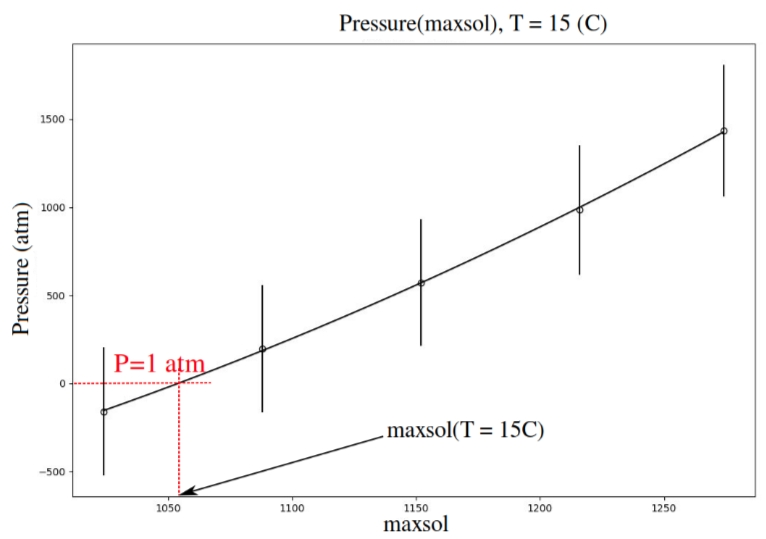
\includegraphics[scale=0.8]{1atm_press_for_maxsol.jpg}}
  \caption{������ ����������� ���������� ����, ����������� � ������������������ (���������� ��������) �������� ��� �������� �����������. ������ ������ �������� ��� ������� �������� � 2-� ������������ ������ ��� $� = 15 C^{\circ}$.}
  \label{img:2:1atm_press_for_maxsol}
\end{figure}

����� ������� �������� ����� ����������� ���������� ���� ��� �������� ����������� � ������� �������. ���������� ���� � ������� -- ���������-��������� ��������, ������� ��� �� ������ �������� �� ����� ��������� ���������� ��� �������� ������ ���-������ ��� ����� ����������. ���������� �� ���� ���������� ���� ����������, ��� �������� �� ���. \ref{img:2:t0_2_conv}, \ref{img:2:t1_0_conv}. �� ���. \ref{img:2:t1_0_conv} ����� ��� �������� ���-������ ������� � 2 ����� ������� ������ ��� ����� ��� ������� 1. �� ����� ����� ���������, ��� ��� ���������� � $1$ ��. ������ ���-������ � 2 ������������ ������ ����������. ���� ���������, ��� ���������� ������� ���������� �� �������� � ����������� �������� ������������ ��� �������� ��������� ������� ������ 2. �� ���. \ref{img:2:t0_2_conv} �����, ��� ������� ������� ���������� �� ������� ����� ��������� ����������� ��� ������ �������� ������. �������� ������� ��������� �� ������� ���������� 1 ��., ������ ��� � ���� ������� ��� <<���������>> ���. \ref{img:2:t1_0_conv}.

\begin{figure}[h!]
  \center{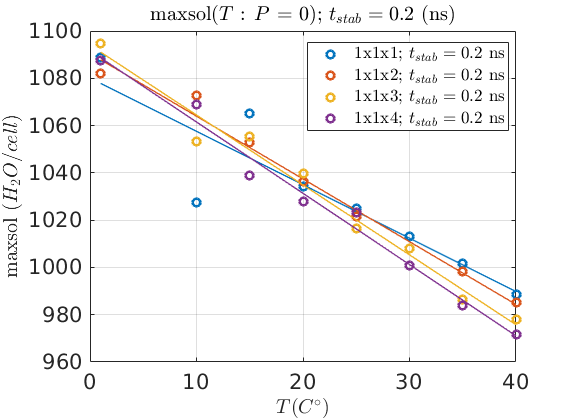
\includegraphics[scale=0.8]{t0_2_conv}}
  \caption{����������� $maxsol$, ������������ ���������� ���. \ref{img:2:1atm_press_for_maxsol}, �� ����������� ��� ��������� �������� ���������� � �������� ��������� �������. ����� ���������� $t_{stab} = 0.2$ ns.}
  \label{img:2:t0_2_conv}
\end{figure}

\begin{figure}[h!]
  \center{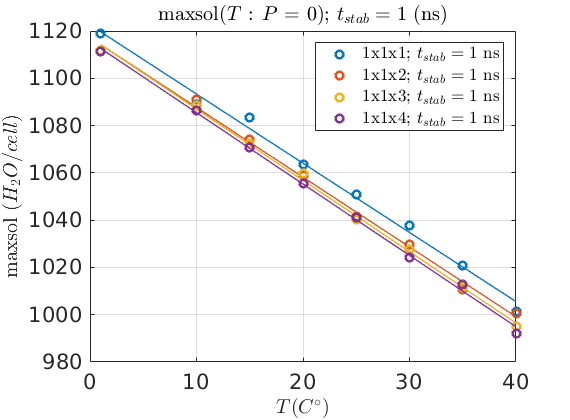
\includegraphics[scale=0.8]{t1_0_conv}}
  \caption{����������� $maxsol$, ������������ ���������� ���. \ref{img:2:1atm_press_for_maxsol}, �� ����������� ��� ��������� �������� ���������� � �������� ��������� �������. ����� ���������� $t_{stab} = 1.0$ ns.}
  \label{img:2:t1_0_conv}
\end{figure}

\newpage

\section{2 ������ ������� ������ ��������� $K$}
\label{Subsec:Calculation2ways}

�������� ���������� �������� ���������� ������� �� ����������, ����� ���������� � ������� ������������ ��� ���������� �������� - ��������� ��������������� ������ ���������.

\begin{equation}
K = - V \left( \dfrac{\partial P}{\partial V} \right)_{T}
\end{equation}

������ ������ \eqref{eq:1:K_explicit}, �������������� � ��������� �������� ������������, ����������� ��� 2 ����� ������ ������ ������� $K$:

\subsection{�������������� �����}

����� �������� \citep{landau2013statistical}, ��� ��� ����������� �� ���������� ��������� �������� ������� + ���������� ($k_B = 1$)

\begin{equation} \label{eq:2:dS_general}
\Delta S_{\Sigma} = - \dfrac{\delta^2 E}{T}.
\end{equation}

���������

\begin{equation}
\begin{aligned}
dE = T dS - P dV + \mu dN \\
\delta = \delta T \dfrac{\partial}{\partial T} + \delta V \dfrac{\partial}{\partial V} + \delta N \dfrac{\partial}{\partial N} \\
\dfrac{\partial (T,S)}{\partial (-P, V)} = \dfrac{\partial (T,S)}{\partial (\mu, N)} = -1 \\
\end{aligned}
\end{equation}

����� �������� 

\begin{equation} \label{eq:2:d2E_general}
\delta^2 E = \delta T^2 \dfrac{\partial S}{\partial T} - \delta V^2 \dfrac{\partial P}{\partial V} + \delta N^2 \dfrac{\partial \mu}{\partial N} + 2 \delta V \delta N \dfrac{\partial \mu}{\partial V}.
\end{equation}

��������� \eqref{eq:2:d2E_general} � \eqref{eq:2:dS_general}. �������� $\delta N = 0$ ��������

\begin{equation} \label{eq:2:exp_dS}
w \sim e^{\Delta S_{\Sigma}} = \exp \left( - \dfrac{\delta^2 E}{T} \right) = \exp \left( - \dfrac{\delta V^2 K}{V T} - \dfrac{\delta T^2}{T} \dfrac{\partial S}{\partial T} \right),
\end{equation}

������ �������� ������� � ��

\begin{equation} \label{eq:2:K_fluct_def}
K_{\sigma^2} = \dfrac{k_B T V}{\langle \Delta V^2 \rangle}
\end{equation}

������ ��� ������� �� \eqref{eq:2:K_fluct_def} ����� �������� � $NPT$ ��������, �.�. ������ �� ������������� ������������ ���������� ������ � ��������� ���������� ������, ��� ���������� ��� ����������� ���������� \eqref{eq:2:exp_dS}.

\subsection{����� ����� ����������}

���� ������ ������������ �� ���. \ref{img:2:dP_dV_idea}: 

\begin{figure}[h!]
  \center{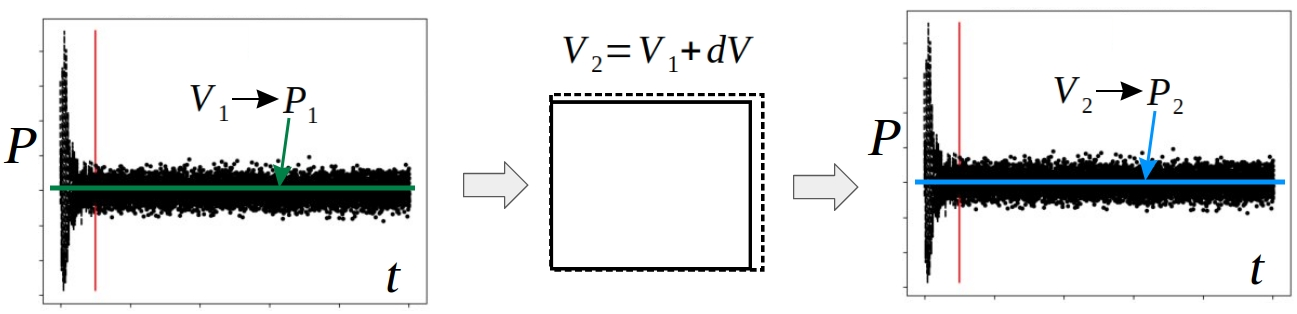
\includegraphics[scale=0.35]{dP_dV_idea}}
  \caption{���� ������� $K$ �� �����������. ������� ������� ��������� �� ���������� � $NVT$ ��������, ����� ������ ������� ������������� � �������, ����� ���� ������� ��������������� �� ����� �������� ��������.}
  \label{img:2:dP_dV_idea}
\end{figure}

�� ����������� $P_1, V_1$, $P_2, V_2$ �������������� 

\begin{equation} \label{eq:2:K_dV_def}
K_{dV} = - \dfrac{V_1 + V_2}{2} \dfrac{P_2 - P_1}{V_2 - V_1}
\end{equation}

� ������ ����� ���� ����� �������� $dV$, ������� �������� �� ������ ��������. ���������� ������ ���������� ���������, ��� ��� � ������������ ������-����������� ������� ���������� ����� �� �������, ������� ����� ������������ �� ����� ������������. ��������� ���������� ��������� ������������ �� ������, �� ������������ �������� ������� $dV / V \ll 1$ �����������. ������ �����, ���������� ������ �������� ���������� �����, ������������ ������������� �������, � �� ����������� ���������. ������� ���������� ������������ ��������, ���������� �� ������� ������� ���������� ���������� ������ �� ������������� �������. ����������, �������� �����������, ����� �����, ���� ��� �������� ������� �� ������ ������ ��� �� ������������ ���������, �.�. ������������ ��������� ����� ������������� ���� ���������� ������������ � �������. ������������ ��������� ����������� ������������. �������������, ����� ����� ���������� ������� �������������� �������� ������ � �������������� �������� ����������, �������� ������������ ����������� ������: $\Delta Q \sim k_B T$. ���������� ����� ����� ����������� ������������� �����������, ��� ����� ����� � � ������������ ���� 

\begin{equation}
\dfrac{\Delta Q}{k_B T} = \dfrac{\alpha \delta L^2}{2 k_B T} \lesssim 1,
\end{equation}

��� $\alpha$ -- ��������� ���������� �����, ������������ ������������ ���������������.

������ $\alpha$ ����������� � �������� ��������, ������� ������ ������� ����������

\begin{equation} \label{eq:2:dL_top_general_final}
\delta L \lesssim \sqrt{\dfrac{2 R T}{\alpha}}.
\end{equation}

��� �������� �������� ���������� ��� ���������� �� 

\begin{equation}
\delta L \lesssim [pm] \sqrt{\dfrac{T / [K]}{20}} \sim 4 pm \hspace{10pt} (T \sim 300K)
\end{equation}

� ������ �������, ��� ������� �� \eqref{eq:2:K_dV_def} �� �������� ������� �������� ��������, ������� ��� ���� ����� ������������. ����� ������� �� ������ �� ������ $\sim 1 / \sqrt{N}$:

\begin{equation}
\Delta P \sim \dfrac{C_1}{\sqrt{t N}} \sim \dfrac{C}{\sqrt{t V}}.
\end{equation}

����� ������ ������� �.�. ���������� ����������, ������������ ��� ��������� $P$, ������� ������ � �������� ������� $V$ � � �������� ���������� $t$. ����� ������� �������� �����, ������� �� ������ �����������, � ������� ����� ��������

\begin{equation}
K = V \dfrac{\delta P}{\delta V}.
\end{equation}

������������ ����������� $\Delta X$ -- ����������� ������� $X$, $\delta X$ -- �������� $X$ ��� ��������� �������.

����� 

\begin{equation}
 \dfrac{\Delta K}{K} = \dfrac{V \delta V}{V \delta P \delta V } \dfrac{C \sqrt{2}}{\sqrt{t V}} = \dfrac{C \sqrt{2}}{\delta P} \dfrac{1}{\sqrt{t V}}.
\end{equation}

��������� ��������� ��������������� �������� �������� $K$, �� ������� ����������� $\delta P \sim K \delta V / V$. �����, ����� � 1 ������� ������������� ��� $\delta V \sim 3 V^{2/3} \delta L$. ����� ��� ���� ����������� �� ��������� ��������

\begin{equation}
\dfrac{\Delta K}{K} = \dfrac{C \sqrt{2}}{K} V^{-1/6} \dfrac{1}{3 \sqrt{t} \delta L} \ll 1.
\end{equation}

��������� ��� � \eqref{eq:2:dL_top_general_final}, �������� ����������� �� ����� ����������

\begin{equation} \label{eq:2:t_avg_condition}
t \gg V^{-1/3} \dfrac{\alpha}{R T} \left( \dfrac{C}{3 K} \right)^2.
\end{equation}

�������� $C$ ����� ������� �� ������ �������. $K = 100$ MPa ��� ������ ���� ����� �� \citep{Gorelov1987} -- ��� ������������� $T \sim 40 C^{\circ}$ � ���� ������� ������ �� \eqref{eq:2:t_avg_condition} ��� ����� ������� $T$, �.�. $K$ ������ � ����������� $T$. � ����� $t > 200$ ��. ��� ������� �������� $1 \times 1 \times 2$ ������������ �����. ��� ���������� ������� ����� ��� ����� ���������, ������� ��� ������������� ������������� ��� �������� ������������ ����� ����������� �������� ������� ���������� � ������� ����������. 
\chapter{���������� �������������}
\label{Sec:Results}

� ���� ����� ��������� ���������� � ������ ��������.

� ������� \ref{Subsec:ResKcompar} ������������ �������� $K$, ���������� ����� ��������, ���������� ����, � ����������������� ��������. ����������� ��������� ������� �����������.

����� � ������� \ref{Subsec:ResWaterMob} ����������� ����������� ������� ����, �.�. ��������� ������ � ��� ����� ������������� ��������� ��������� ��������� $K$ � ������������.

����� � \ref{Subsec:ResWater2phase} �������� ����������� ��������� ���� �� ���������� ����, ����������� � �������. �� ��� ����� ���������� ���������� ����, ����������� ��� ��������������� ������������ � �������� ����������


\section{��������� ��������� � ����������������� $K$}
\label{Subsec:ResKcompar}

\subsection{����������� ������ ������� ������� $K$}

������� ��� ��������� ������ \eqref{eq:2:K_dV_def} � \eqref{eq:2:K_fluct_def} ��� <<�������>> ������� ����+�����, ���� ��������� �� �� ����� ������� �������. �������� ��� ���� ������ �������� ����������������� �������� $K$. � ���� ��, ���� ����� ����������� � � ������� �������, ������� ��������� �� ���������� ��������������� ���� �� � ������ ���� ��� ����� ����������. ���, ��� � �����, ������������ ������ ���� tip4p/2005 \citep{Abascal2005}. ����� � ������ ����� ������� ������ ���� ������ ����� ������������ � ���������� ������ SPC/E � tip3p ������ ������, ��� ������ ����� $K$ ��� ���������� ����������� ����������� �� ��������� $\sim 10 K$, � �� ����� ��� ���� ����� ����� ������ �������� ��� �������� ����������� ������������� ���� ���������� ������� SPC/E �� $\sim 50K$. 

�� ���. \ref{img:3:water_test_2methods} ��������� ��������� ������������������ $K$ � ������������� �� \eqref{eq:2:K_dV_def} � \eqref{eq:2:K_fluct_def}. �������������� ����� ��������� � ������������� � �������� �����������, �� ��� ����������� ���������� ������ $\sim 10\%$. ����� ����� �������� ���� ������� �����������, � ���� ���������� �� ������������ �� $\sim 5\%$. 

� ������������� �������� ����� ���������� ������, ������ ���� � \eqref{eq:2:t_avg_condition} �� ��������, ��� ����� ����������, ����������� ��� ������� ������ ������ ����� ��������, ����������� ��� $t > 200$ ��., � ����� �� �������, ��� ��� ���������� $\sim 1$ ��. ����������� ��� ���������� $\sim 5\%$. ���� � ���, ��� ������ \eqref{eq:2:t_avg_condition} ���� �������� �� ����������� �� ������� ��������, ���������� �� ��������� ������� ���������� ���������� ������ � ����� � ������������. � ������ �� ������ ���� �������� ����� ���� ������� ������, �.�. ������� �� ������� ������� ������� ��� ����� ������ ������ � ���������� ���� ����� �������� ����������. � ������ ����� ���� ������ �������� ������� ������ ��� \eqref{eq:2:dL_top_general_final}, ��� ���� ������� ������� ��������� �������� � �������, ��� � ���� ������� ��������� ������������� ����������� ������� $K$.

\begin{figure}[h!]
  \center{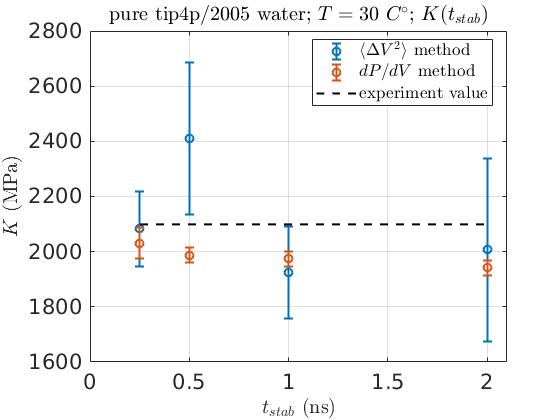
\includegraphics[scale=0.5]{water_test_2methods}}
  \caption{��������� $K$, ���������� 2 ������� �������� \eqref{eq:2:K_dV_def} � \eqref{eq:2:K_fluct_def}, � ������������������ ����������.}
  \label{img:3:water_test_2methods}
\end{figure}

\subsection{���������� $K$ �� ���������� ���������� � ���������}



\section{������ ����������� ������� ����}
\label{Subsec:ResWaterMob}

2

\section{2-������ ������������� ��� ����� ���������}
\label{Subsec:ResWater2phase}

3

\conclusion

В ходе выполнения данной работы:

\begin{itemize}
\item Сформулирован алгоритм проготовки кристалла к MD-расчету. 

\item Проверены сходимости по параметрам системы. 

\item Реализовано 2 независимых метода расчета К кристалла. К, расчитанные по этим 2 методам, согласуются между собой, но плохо согласуются с экспериментом.

\item Проанализирована модильность молекул воды в белке.

\item Проведено сравнение результатов при различных моделях воды.

\item Лизоцим стабилизирован при различных влажностях с использованием 2-фазного моделирования.  

\item Найден приближенный диапазон влажности, оптимальный для расчета модуля упругости. 

\item В дальнейшем планируется провести расчет $K$ при различных влажностях. Так же возможно проведение расчетов с другими параметризациями белка для улучшения совпадения с экспериментом.

\end{itemize}



\bibliography{DyachkovBibliography}
\bibliographystyle{gost705}

%\appendix
%\input{app-a}

\end{document}
